\chapter{Implementierung und Design}
\label{sec:implementation}
In diesem Kapitel der Arbeit wird die Implementierung auf Basis der aufgestellten Anforderungen in Kapitel \ref{sec:requirements} betrachtet. Die Verzeichnisstruktur, auf welche in den folgenden Kapiteln eingegangen wird, ist als Baumstruktur mit Abbildung \ref{fig:dirstructure} gegeben. Die gesamte Applikation befindet sich auf dem Repository im Verzeichnis \texttt{app}. Da die allgemeine Architektur (vgl. Abbildung \ref{fig:architecture}) mithilfe der Containervirtualisierung über Docker aufgebaut ist, wird zunächst dieser Aspekt erläutert. Im Anschluss findet jeweils eine Unterscheidung zwischen der Architektur für das Front-End und das Back-End statt.

\begin{figure*}[t]
    \centering
    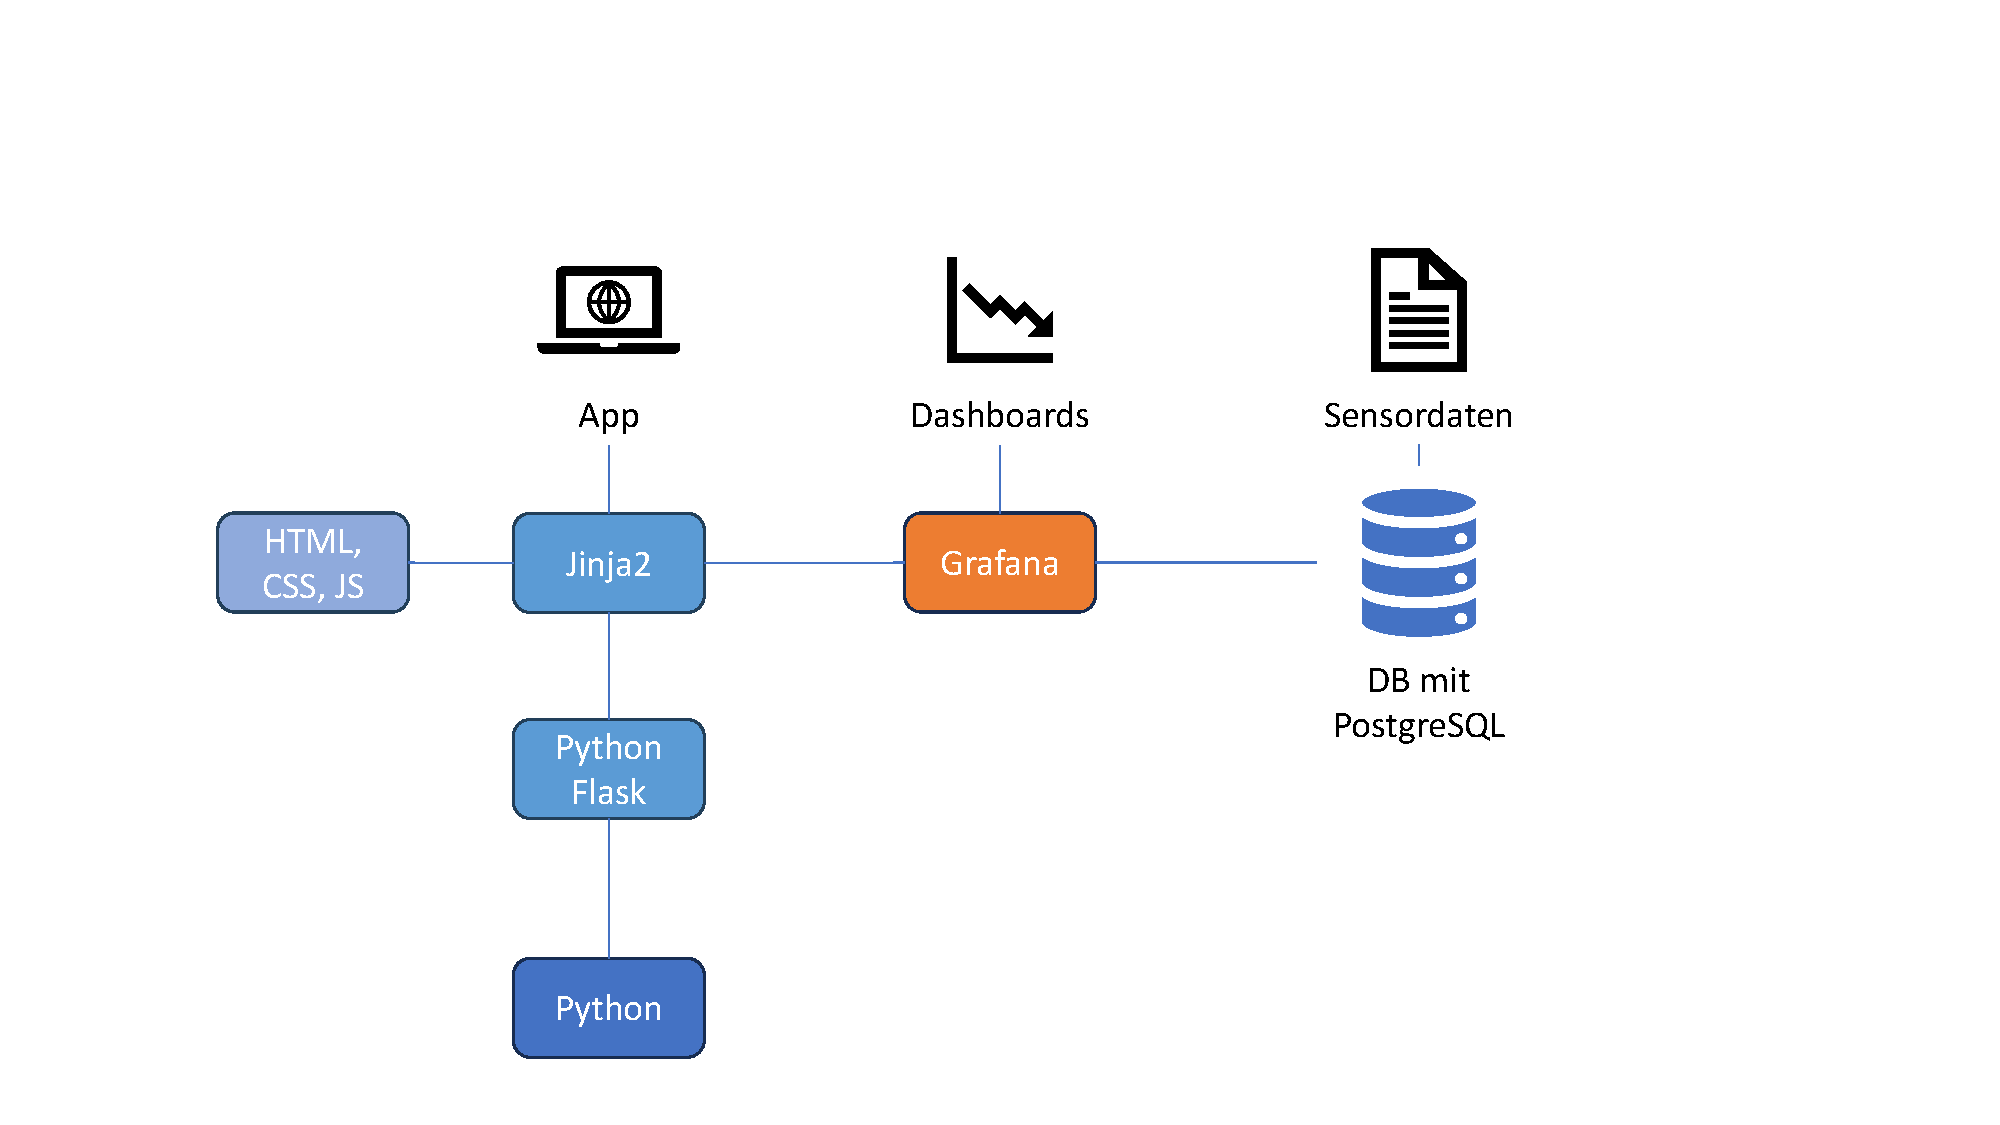
\includegraphics[width=\widefigurewidth]{appendices/Architektur.pdf}
    \caption[Architektur]{Die vorliegende Architektur für die Applikation}
    \label{fig:architecture}
\end{figure*}

\begin{marginfigure}
    \centering
    \begin{adjustbox}{width=\textwidth}
        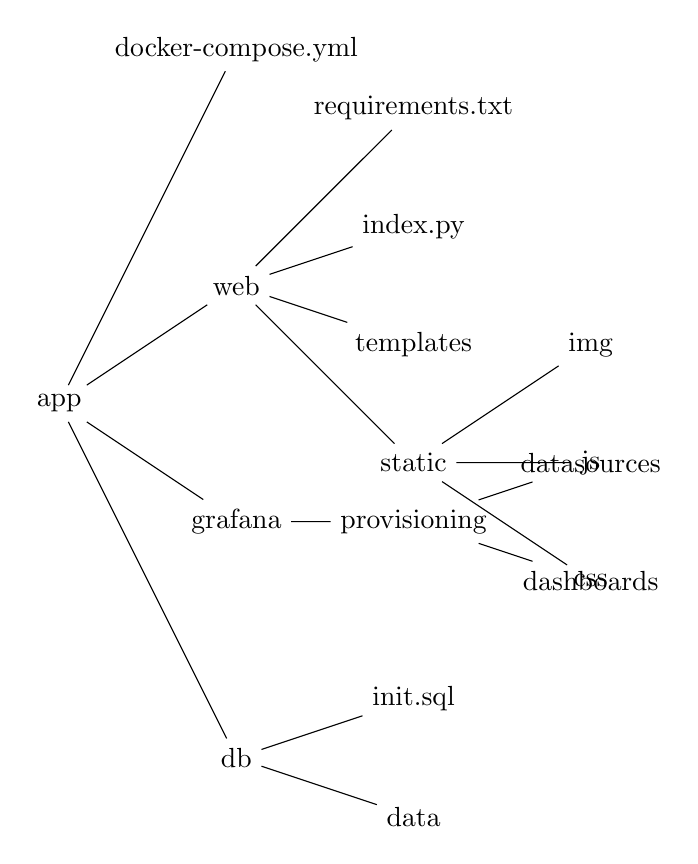
\begin{tikzpicture}[
                grow=right,
                scale=1.5,
                level 1/.style={sibling distance=2cm},
                level 2/.style={sibling distance=1cm}
            ]
            \node{app}
            child { node {db}
                    child { node {data}}
                    child { node {init.sql}}}
            child { node {grafana}
                    child { node {provisioning}
                            child { node {dashboards}}
                            child { node {datasources}}
                        }
                }
            child { node {web}
                    child { node {static}
                            child { node {css}}
                            child { node {js}}
                            child { node {img}}}
                    child { node {templates}}
                    child { node {index.py}}
                    child { node {requirements.txt}}
                }
            child { node {docker-compose.yml}};
        \end{tikzpicture}
    \end{adjustbox}
    \caption{Die Verzeichnisstruktur der Applikation}
    \label{fig:dirstructure}
\end{marginfigure}

\section{Containervirtualisierung mit Docker}
Aufgrund der Tatsache, dass ein privater Entwickler ein Produktivsystem mit mehreren Komponenten simulieren muss, hat sich der Einsatz Dockers als sinnvoll erwiesen. Docker ist eine Open-Source-Software, die es ermöglicht, Anwendungen mithilfe von Containervirtualisierung zu isolieren. Dabei wird die Anwendung in einem Container ausgeführt, der alle Abhängigkeiten enthält, die für die Ausführung der Anwendung erforderlich sind. Die Container sind dabei leichtgewichtiger als virtuelle Maschinen, da sie den Kernel des Host-Betriebssystems nutzen\sidenote{\url{https://www.docker.com/resources/what-container/}}. Für diese Arbeit sind drei Anwendungen notwendig: eine Python-Flask Instanz für einen Webserver (Port 5000), eine PostgreSQL-Instanz für die Datenbank (Port 5432) und eine Grafana-Instanz (Port 3000) für die Verarbeitung und Visualisierung der Daten aus der Datenbank. Diese drei Anwendungen werden jeweils in einem eigenen Container ausgeführt und einem Netzwerk zugewiesen, um eine Kommunikation zwischen den Containern zu ermöglichen (vgl. Abbildung \ref{fig:dockerarchitecture}). Diese notwendigen Eigenschaften werden in einer \texttt{docker-compose.yml}-Datei definiert. Diese Datei wird von Docker verwendet, um die Container zu erstellen und zu starten. Die \texttt{docker-compose.yml}-Datei befindet sich im Hauptverzeichnis der Applikation.

\begin{figure*}[t]
    \centering
    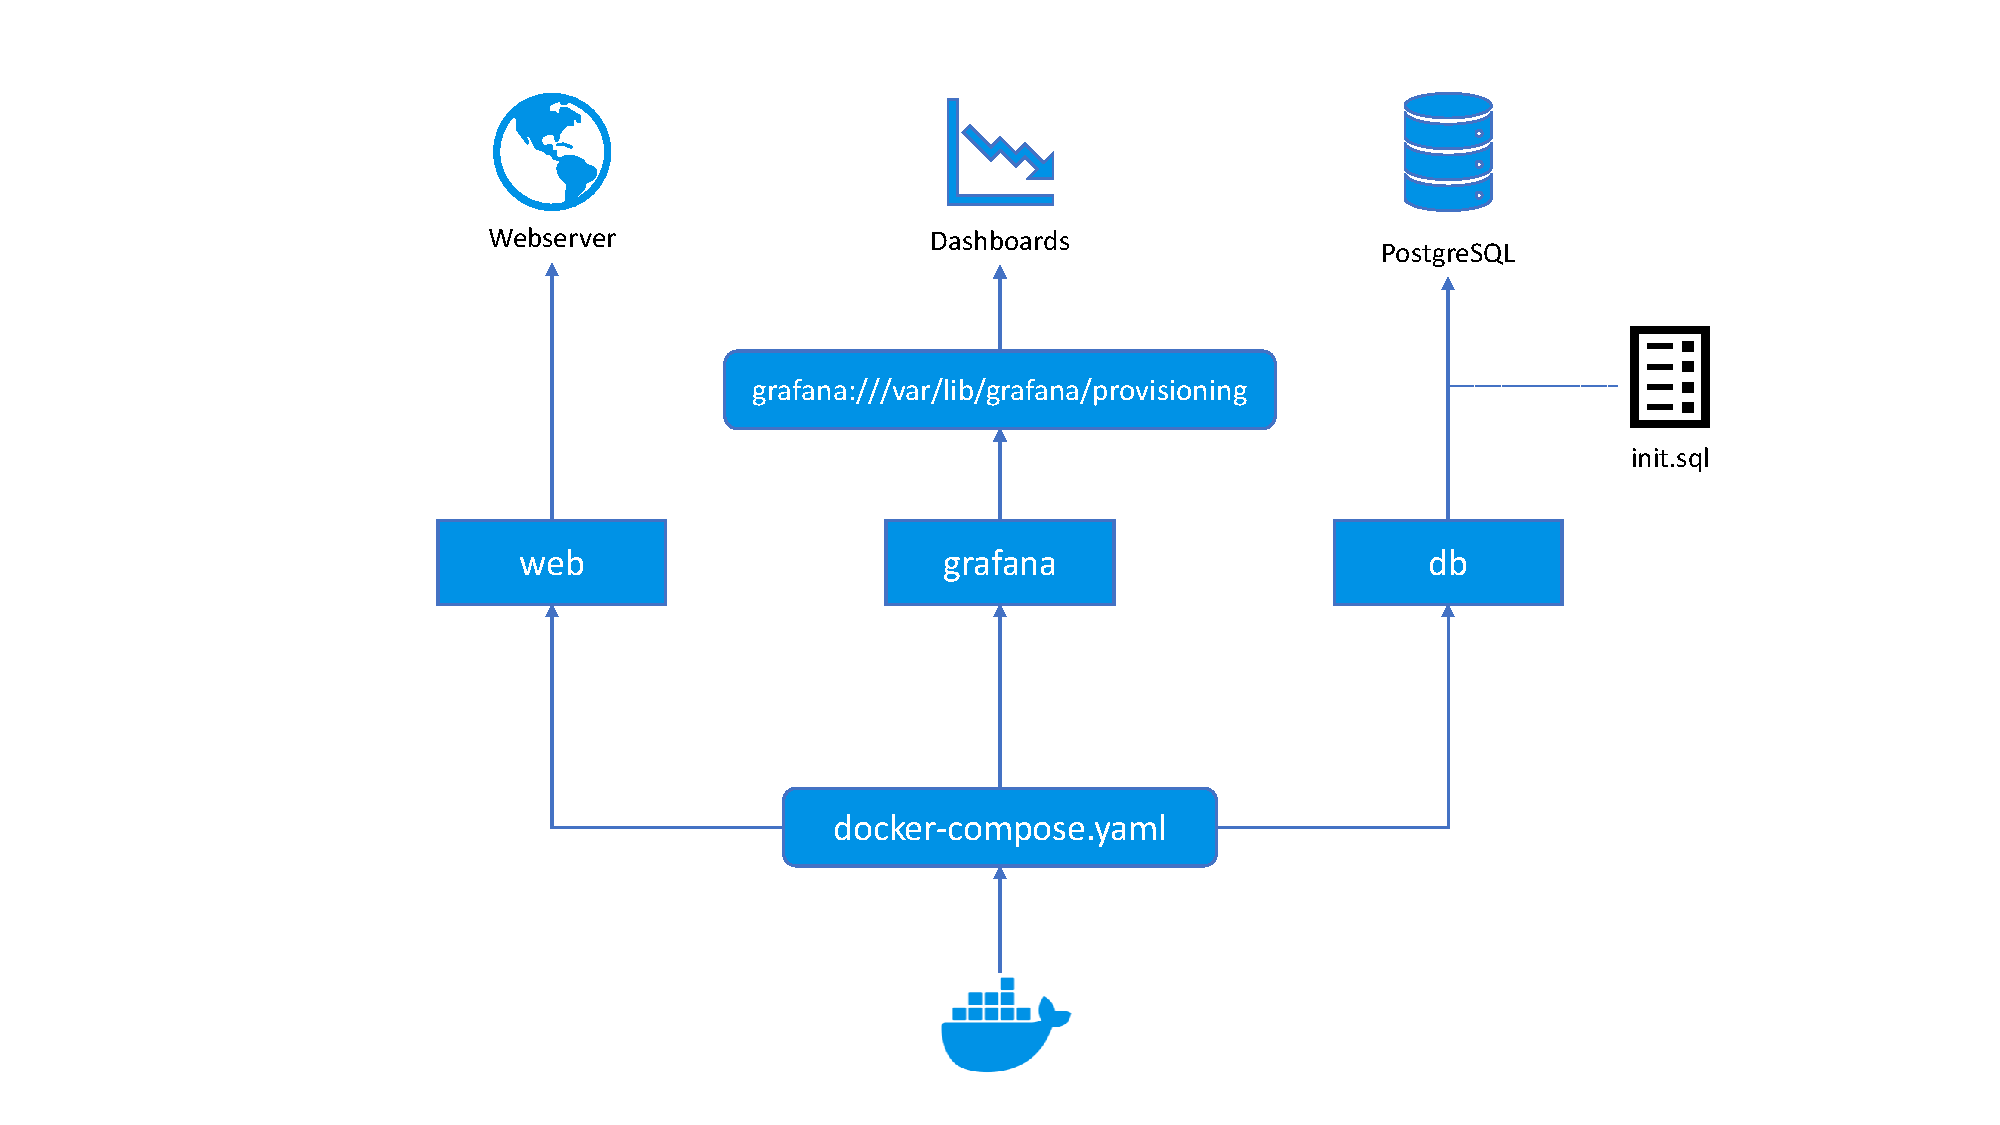
\includegraphics[width=\widefigurewidth]{appendices/Architektur_Docker.pdf}
    \caption[Docker-Architektur]{Die vorliegende Docker-Architektur für die Applikation}
    \label{fig:dockerarchitecture}
\end{figure*}

\section{Architektur für das Front-End}
Das Front-End der Applikation ist mit dem Web-Framework Python-Flask\sidenote{\url{https://flask.palletsprojects.com/}} und den daraus resultierenden Komponenten umgesetzt. Die Wahl, welche Programmiersprache zur Implementierung des Werkzeugs zum Einsatz kommen soll, ist auf Python\sidenote{\url{https://www.python.org/}} gefallen, da es sich um eine leichtgewichtige und einfach zu erlernende Sprache handelt. Zudem ist Python eine der beliebtesten Programmiersprachen\sidenote{\url{https://spectrum.ieee.org/top-programming-languages-2022}} und bietet daher eine umfangreiche Dokumentation zum Umsetzen der individuellen Anforderungen. Flask verwendet als Template-Engine Jinja2\sidenote{\url{https://jinja.palletsprojects.com/}}, mit dessen Hilfe HTML- und JavaScript-Code, als auch CSS-Stylesheets eingebunden werden können. Alle Webserver-Komponenten befinden sich im Verzeichnis \enquote{web}. Innerhalb dieses Verzeichnisses ist folgende Unterteilung vorzufinden:

\begin{itemize}
    \item \textbf{templates} für alle HTML-Dateien, die als Templates für die Jinja2-Engine dienen. In diesem Verzeichnis befindet sich die \texttt{base.html}, welche die Grundlage für alle anderen HTML-Dateien darstellt. In dieser Datei werden alle notwendigen Komponenten wie Stylesheets, JavaScript-Code und die Navigation eingebunden. Die anderen HTML-Dateien erben von dieser Datei und können somit auf die Komponenten zugreifen. TODO: VERWEIS AUF ANHANG
    \item \textbf{static} für alle statischen Dateien, wie CSS-Stylesheets und Bilder (z.B. Favicons für Logos). Auch JavaScript-Dateien werden hier abgelegt um Unterverzeichnisse simpler zu gestalten, obwohl es sich hier um eine dynamische Programmiersprache handelt.
    \item \textbf{index.py} für die Python-Flask-Instanz, die den Webserver darstellt. In dieser Datei werden alle Routen definiert, die der Webserver bereitstellen soll. Das Session- und Cookie-Handling, HTTP-Requests und -Responses und das Logging können ebenfalls in dieser Datei definiert werden.
    \item \textbf{requirements.txt} für alle Python-Abhängigkeiten, die für die Ausführung der Applikation notwendig sind. Diese Datei wird von Docker verwendet, um die Abhängigkeiten zu installieren.
\end{itemize}

Zum Visualisieren und Interagieren der Daten kommt die Open-Source-Software Grafana\sidenote{\url{https://grafana.com/}} zum Einsatz. Mithilfe von Grafana lassen sich Daten aus einer Datenbank abrufen (vgl. \ref{sec:backend}), individuell visualisieren und in Dashboards einpflegen (vgl. Abbildung \ref{fig:grafana}). Zu Visualisierungszwecken befinden sich acht Dashboards in der Sammlung der Bamberger Wetterstationen, wobei es sich bei einem Dashboard um die Zusammenlegung der anderen sieben Wetterstationen handelt, um einen Vergleich zwischen diesen zu ermöglichen. Der Fokus liegt dabei auf der Visualisierung der Temperatur zu einer gegebenen Uhrzeit für jede Wetterstation. Mithilfe von Grenzwerten, die in den Dashboards definiert werden können, lassen sich Temperaturbereiche farblich\sidenote{Die Farbe Blau soll repräsentativ für kalte Temperaturen sein, während die Farbe Rot hohe Temperaturen symbolisieren soll} hervorheben. Der Aspekt des Crowdsensings wird nativ von Grafana durch die Möglichkeit, einen Punkt auf dem Graphen zu markieren und eine Annotation an diese Markierung hinzuzufügen, unterstützt. Diese Annotationen sollen dann durch andere Nutzer*innen des Werkzeuges eingesehen werden können.

Das Front-End bietet mehrere Seiten an, zwischen jenen mithilfe des Routings navigiert werden kann:

\begin{itemize}
    \item \textbf{Home} für die Startseite der Applikation. Hier werden alle Wetterstationen und die definierten \ac{LCZ} auf einer OpenStreetMap\sidenote{\url{https://www.openstreetmap.org/}}-Karte eingeblendet. Auf der rechten Seite haben die Nutzer*innen mithilfe eines Chatfensters die Möglichkeit, sich mit anderen Nutzer*innen zu den Daten auf der Karte auszutauschen.
    \item \textbf{Sensorinspektor} für die Analyse der Daten aus den Bamberger Wetterstationen. Auf dieser Seite werden die Daten aus Grafana mithilfe von iFrames\sidenote{HTML-Tag zum Einbetten von anderen Dokumenten in eine HTML-Datei} eingebunden und durch Filtermöglichkeiten (zu Wetterstationen, Datum und Uhrzeit) mithilfe von Dropdown-Menüs eingeschränkt.
    \item \textbf{Feedback} für die Möglichkeit, Feedback zu der Applikation zu geben. Hier können die Nutzer*innen eine Nachricht hinterlassen und dieser eine Kategorie zuweisen (Fehlermeldung, Änderungsvorschlag oder neues Feature).
    \item \textbf{User} für die Benutzerverwaltung. Hier ist es möglich, sich zu registrieren und anzumelden. Nach der Anmeldung können die Nutzer*innen ihr Profil, ihre Chats und ihr Feedback einsehen.
\end{itemize}

\begin{marginfigure} % [t]: place at top of page (recommended)
    \centering
    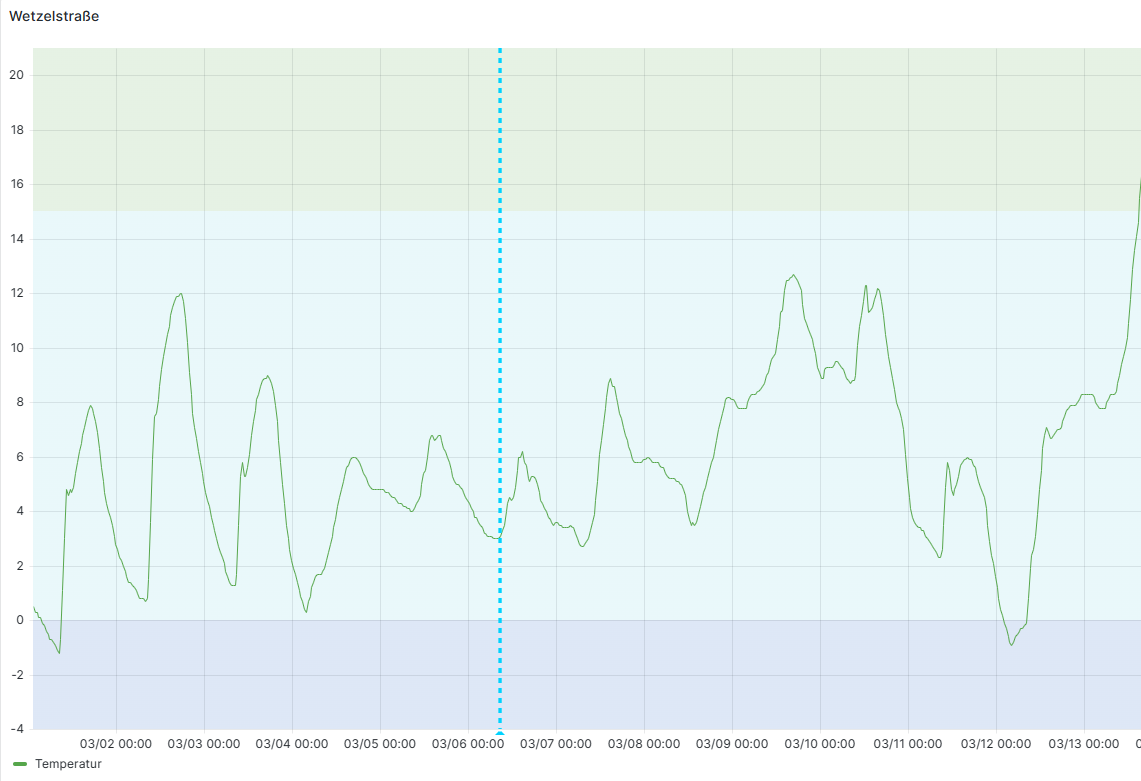
\includegraphics[width=1\textwidth]{figures/grafana.png}
    \decoRule
    \caption[Grafana-Dashboard]{Repräsentatives Grafana-Dashboard mit den Sensordaten aus der Wetzelstraße in Bamberg}
    \label{fig:grafana}
\end{marginfigure}

\section{Architektur für das Back-End}
Das Back-End der Applikation ist mit PostgreSQL\sidenote{\url{https://www.postgresql.org/}} als relationales Datenbankmanagementsystem umgesetzt. Die Wahl, welche Datenbank zum Einsatz kommen soll, ist auf PostgreSQL gefallen, da es sich um Open-Source-Software handelt, eine einfache Einbindung in Grafana möglich ist und PostgreSQL eine umfangreiche Dokumentation zur Verfügung stellt. Zusätzlich entspricht PostgreSQL weitestgehend dem SQL-Standard. \\ Eine Stichprobe\sidenote{Zwischen dem 01. März 2023 und 10. August 2023} der Sensordaten der Wetterstationen in Bamberg wird durch eine parallel laufende Abschlussarbeit am \ac{MOBI-Lehrstuhl} in Form von CSV\sidenote{Comma-separated values, häufiges Dateiformat zum Austausch von Daten}-Dateien zur Verfügung gestellt. Diese Daten werden von Docker Compose beim Starten der Container aus dem Verzeichnis \texttt{db/data} in die Datenbank importiert und durch SQL-Befehle in der Datei \texttt{db/init.sql} in die Datenbank eingefügt (vgl. Abbildung \ref{lst:sqlcode}). \\ Im Anschluss liegt die Tabelle \texttt{stations} in der Datenbank mit folgenden Spalten vor:

\begin{lstlisting}[language=SQL,float=t,
      caption={SQL-Befehle zum Erstellen der Tabelle \texttt{stations} in der Datenbank},label={lst:sqlcode}]
      CREATE TABLE stations (
        id SERIAL PRIMARY KEY,
        p_id INT,
        time TIMESTAMP,
        station VARCHAR(50),
        ta FLOAT,
        lon FLOAT,
        lat FLOAT,
        z INT,
        humidity FLOAT
      );
      
      COPY stations(p_id, time, station, ta, lon, lat, z, humidity) FROM '/data/Bamberg_Stations 01.03.2023to31.03.2023.csv' DELIMITER ';' CSV HEADER;
      COPY stations(p_id, time, station, ta, lon, lat, z, humidity) FROM '/data/Bamberg_Stations 01.04.2023to30.04.2023.csv' DELIMITER ';' CSV HEADER;
      COPY stations(p_id, time, station, ta, lon, lat, z, humidity) FROM '/data/Bamberg_Stations 01.06.2023to30.06.2023.csv' DELIMITER ';' CSV HEADER;
      COPY stations(p_id, time, station, ta, lon, lat, z, humidity) FROM '/data/Bamberg_Stations 01.07.2023to31.07.2023.csv' DELIMITER ';' CSV HEADER;
      COPY stations(p_id, time, station, ta, lon, lat, z, humidity) FROM '/data/Bamberg_Stations 01.08.2023to10.08.2023.csv' DELIMITER ';' CSV HEADER;
      
\end{lstlisting}

\begin{itemize}
    \item \textbf{id} ist notwendig als Primary Key, um die Daten eindeutig zu identifizieren.
    \item \textbf{p\_id} als ID der Wetterstation.
    \item \textbf{time} als Zeitstempel.
    \item \textbf{station} als Name der Wetterstation.
    \item \textbf{ta} als Temperatur in Grad Celsius.
    \item \textbf{lon} als Längengrad.
    \item \textbf{lat} als Breitengrad.
    \item \textbf{z} als Höhe über dem Meeresspiegel.
    \item \textbf{humidity} als Luftfeuchtigkeit in \%.
\end{itemize}

Mit dieser Struktur ist es nun möglich, die Auslesungen der Wetterstationen für einen Zeitpunkt abzufragen. Außerdem bietet die Spalte \texttt{station} die Möglichkeit, nach einer bestimmten Wetterstation zu filtern. Auf diese Weise können die Daten aus der Datenbank in Grafana eingespeist werden.

\label{sec:backend}